\section{Discussion}
\begin{frame}{Discussion}{Jesper F. Hansen}


\begin{itemize}
    \item Results of the simulations
    \item Inaccuracies in simulations
    \begin{itemize}
        \item Motion of the manipulator
        \item No physical forces
    \end{itemize}
\end{itemize}
\begin{table}[]
    \centering
\begin{tabular}{l l l}
    \hline
    \rowcolor{beamer@barcolor}\textbf{Requirement} & \textbf{Result} \\
    \hline
    Workcell dimensions & Simulated \\
    \rowcolor{beamer@barcolor} Workcell Safety & Simulated \\
    Material flow & Simulated \\
    \rowcolor{beamer@barcolor} Cycle time & Failed \\
    \hline
\end{tabular}
\end{table}
\end{frame}

\begin{frame}{Discussion}{Testing}
\begin{itemize}
    \item Results from testing
    \item Inaccuracies in testing
    \begin{itemize}
        \item UR5 vs KUKA KR 6 R700 sixx
        \item Laser Pointer
        \item CAD model
        \item Script
    \end{itemize}
\end{itemize}
\begin{table}[]
    \centering
    \begin{tabular}{l l l}
        \hline
        \rowcolor{beamer@barcolor}\textbf{Requirement} & \textbf{Result} \\
        \hline
        Industrial manipulator & Succeeded \\
        \rowcolor{beamer@barcolor}Constant velocity & Failed \\
        Relative distance & Succeeded\\
        \rowcolor{beamer@barcolor}Perpendicular angle & Succeeded\\
        $30.0\degree$ angle & Succeeded \\
        \rowcolor{beamer@barcolor}Deviation & Failed \\
        \hline
    \end{tabular}
\end{table}
\end{frame}

\section{Conclusion}
\begin{frame}{Conclusion}
% \begin{alertblock}{
\begin{center}
Therefore, it can be concluded that without further improvements, the \textit{CORPS} is not a feasible solution for implementation in \textit{Grundfos}’ production line.
\end{center}
% }\end{alertblock}%%%%%Is this the way to use alert? If so....I don't like it..%%%%%%
\end{frame}

\section{Future Work}
\begin{frame}{Future Work}{Improvements}
\begin{columns}
\column{.45\textwidth}
\begin{itemize}
    \item Number of points
    \item Position and orientation
    \begin{itemize}
    % from 08.810 to 40.930 = $32.120$ $s$
        \item From $32.1$ $s$ to $9$ $s$
    \end{itemize}
\end{itemize}
\column{.55\textwidth}
\begin{center}
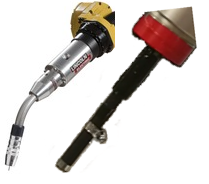
\includegraphics[width=0.815\textwidth]{graphics/jesper/pointer_n_weldgun}

\tiny{(lincolnelectric.com)}
\end{center}
\end{columns}
\end{frame}

\begin{frame}{Future Work}
\begin{itemize}
    \item Sustainability and stakeholders
    \item Simulation
    \item Elimination of inaccuracies
\vspace{4mm}
\item Alternative solutions:
\begin{itemize}
    \item Turning impeller
    \item Spot weld
\end{itemize}
\end{itemize}
\end{frame}

\section{Process Analysis}
\begin{frame}{Process Analysis}{Collaboration}
\begin{itemize}
    \item Group
    \begin{itemize}
        \item Good intentions
        \item Misunderstandings and bad communication
        \item What we could have done
        \begin{itemize}
            \item Belbin and Felder
            \item Conflict tools
            \item Supervisors
        \end{itemize}
    \end{itemize}
    \item Supervisors
    \begin{itemize}
        \item Loose contract
        \item Beneficial collaboration
    \end{itemize}
\end{itemize}
\end{frame}

\begin{frame}{Process Analysis}{Project Management}
\begin{itemize}
    \item Timetable
    \item Scrum board
    \item Daily meetings
    \item Laboratory schedule
\end{itemize}
\end{frame}

\begin{frame}{Process Analysis}{Learning process}
\begin{itemize}
    \item Learning process
    \begin{itemize}
        \item P2 project
        \item Peer learning
        \item Group sessions
    \end{itemize}
\end{itemize}
    
\end{frame}